\section{Ejercicio 9}

Para este ejercicio se pedía implementar el scheduler \textit{Multilevel Feedback Queue}, realizar pruebas y mostrar su ejecución.

\subsection{Implementación}

Este scheduler posee n colas \emph{Round Robin} y a cada una de ellas le está asociado un quantum. Estos son recibidos como parámetro.

La estructura que utilizamos es la siguiente:

		vector<int> quantums_por_cola; //El quantum que corresponde a cada cola
		vector< queue<proceso*> > colas_de_procesos; //Vector de colas de procesos
		vector<proceso*> proceso_en_core; //Procesos corriendo
		vector<proceso*> proceso_bloqueado; //Procesos bloqueados

\begin{itemize}

\item \textbf{quantums\_por\_cola}: vector que posee el quantum que corresponde a cada cola.

\item \textbf{colas\_de\_procesos}: vector de colas donde las de mayor prioridad se encuentran en los primeros índices y las de menor en los últimos.

\item \textbf{proceso\_en\_core}: vector que toma como índice el core que tiene un puntero al proceso que le corresponde

\item \textbf{proceso\_bloqueado}: vector de punteros a procesos que fueron bloqueados

\end{itemize}

En el constructor se inicializa el vector \textbf{proceso\_en\_core} con la cantidad de cores recibidos por parámetro y inicializamos los vectores \textbf{colas\_de\_procesos} y \textbf{quantums\_por\_cola}. Mientras haya quantums en el vector que se recibe como parámetro se van agregando colas a \textbf{colas\_de\_procesos} y el quantum en \textbf{quantums\_por\_cola}.

En la función \textbf{load}, el nuevo proceso es cargado en la cola de mayor prioridad (índice 0) de \textbf{colas\_de\_procesos}.

En la función \textbf{unblock}, se busca el proceso en el vector \textbf{proceso\_bloqueado} para volverlo a insertar en \textbf{colas\_de\_procesos} con su prioridad elevada.

La función \textbf{tick} tiene un comportamiento mas complejo que pasamos a detallar en el siguiente pseudocódigo:

~

\begin{algorithmic}
\Function{int tick}{int cpu, const enum Motivo m}

	\If {\emph{Si la tarea actual es la IDLE\_TASK y hay procesos en alguna cola}}
		\State Desencolo el proceso de cola de mayor prioridad.
		\State Agrego el proceso al core.
		\State Lo devuelvo.
		
	
	\ElsIf{\emph{Si el motivo fue un TICK}}
		\State Actualizo el quantum de la tarea.

		\If{\emph{Si terminó su quantum}}
			\State Quito el proceso de \textbf{proceso\_en\_core}. Y lo encolo en la siguiente cola con menor prioridad.
			\State Tomo un nuevo proceso de la cola de mayor prioridad, lo agrego al vector \textbf{proceso\_en\_core} y lo devuelvo.
		\EndIf

	\ElsIf{\emph{Si el motivo fue un EXIT}}
		\State Elimino el proceso que termino.
		\State Tomo un nuevo proceso de la cola de mayor prioridad, lo agrego al vector \textbf{proceso\_en\_core} y lo devuelvo.

	\ElsIf{\emph{Si el motivo fue un BLOCK}}
		\State Agrego el proceso al vector \textbf{proceso\_bloqueado}
		\State Tomo un nuevo proceso de la cola de mayor prioridad, lo agrego al vector \textbf{proceso\_en\_core} y lo devuelvo.
	
	\EndIf
\EndFunction	
\end{algorithmic}

\subsection{Pruebas}

Para estas pruebas generamos un lote (\textit{ej9lote}) que posee cinco tareas de los tipos TaskCPU, TaskConsola, TaskBatch y TaskAlterno, elegimos este lote para estudiar como se comporta con tareas que hacen uso intensivo del CPU y tareas interactivas que realizan llamadas bloqueantes. Estas son lanzadas desde el comienzo con una diferencia de dos clocks cada una. La cantidad de cores es de uno, el costo del cambio de contexto es de dos y el costo de cambiar un proceso de núcleo es de uno.

En este caso, tenemos tres colas de quantums crecientes (8, 10 y 12), crecientes (4, 6 y 8) y (1, 2, 3). Veamos cómo se comportan:

\begin{figure}[!h]
	\begin{center}
		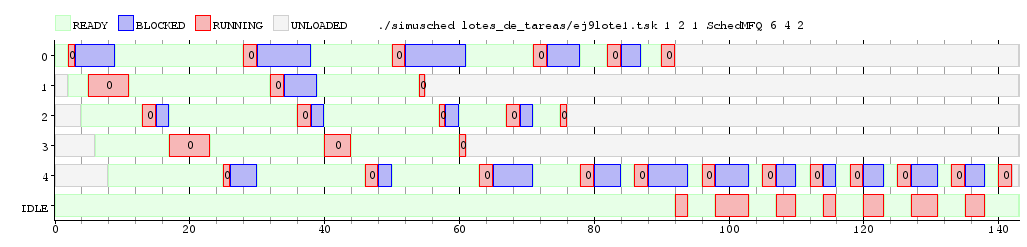
\includegraphics[width=500px]{imagenes/ej9_1.png}
		\caption{Ejecución del lote \emph{ej9lote} con tres colas de quantum decreciente.}
		\label{fig:grafico_ej9_1}
	\end{center}
\end{figure}

\begin{figure}[!h]
	\begin{center}
		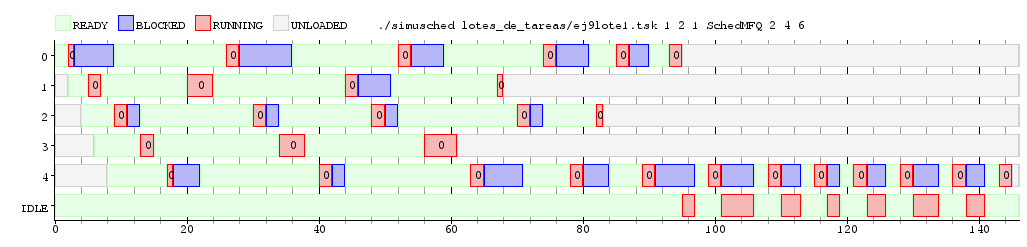
\includegraphics[width=500px]{imagenes/ej9_2.png}
		\caption{Ejecución del lote \emph{ej9lote} con tres colas de quantum creciente.}
		\label{fig:grafico_ej9_2}
	\end{center}
\end{figure}

\begin{figure}[!h]
	\begin{center}
		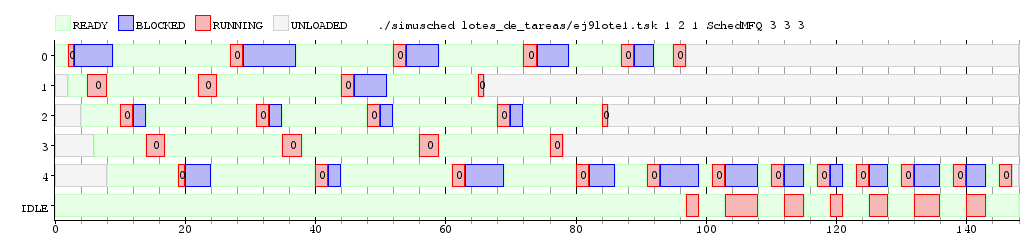
\includegraphics[width=500px]{imagenes/ej9_3.png}
		\caption{Ejecución del lote \emph{ej9lote} con tres colas con quantum 3.}
		\label{fig:grafico_ej9_3}
	\end{center}
\end{figure}

%LATENCIA PROMEDIO
\begin{center}
	\begin{tabular}{|c|c|c|}
		\hline
		\multicolumn{3}{|c|}{\large{\textbf{Latencia Promedio}}} \\
		\hline
		\textbf{Quantum Decreciente} & \textbf{Quantum Creciente} & \textbf{Quantum Estable} \\
		\hline
		8,4 & 5,2 & 6 \\
		\hline
	\end{tabular}
\end{center}

%WAITING TIME PROMEDIO
\begin{center}
	\begin{tabular}{|c|c|c|}
		\hline
		\multicolumn{3}{|c|}{\large{\textbf{Waiting Time Promedio}}} \\
		\hline
		\textbf{Quantum Decreciente} & \textbf{Quantum Creciente} & \textbf{Quantum Estable} \\
		\hline
		50,2 & 57,4 & 58 \\
		\hline
	\end{tabular}
\end{center}

%TIEMPO TOTAL DE EJECUCION PROMEDIO
\begin{center}
	\begin{tabular}{|c|c|c|}
		\hline
		\multicolumn{3}{|c|}{\large{\textbf{Tiempo Total De Ejecución Promedio}}} \\
		\hline
		\textbf{Quantum Decreciente} & \textbf{Quantum Creciente} & \textbf{Quantum Estable} \\
		\hline
		81,6 & 86,4 & 90,6 \\
		\hline
	\end{tabular}
\end{center}

Cómo podemos observar en esta prueba, tener un quantum decreciente hace que la latencia sea la mayor, pero genera un waiting time y tiempo total de ejecución menores que las otras dos ejecuciones con quantum creciente y quantum estable. Tener un quantum creciente genera que su latencia promedio sea la menor pero con waiting time promedio y tiempo de ejecución promedio mucho mayores. Tener un quantum estable genera que este scheduler sea cómo un \textbf{Round Robin} común ya que no se diferencian las prioridades de las colas que pueda poseer.

Este scheduler resulta interesante para analizar y comparar contra los otros schedulers vistos en este trabajo ya que podría mejorar la performance de estos. 
